% vim: set textwidth=78 autoindent:

\section{4. Δημιουργώντας PyQGIS εφαρμογές}

% when the revision of a section has been finalized, 
% comment out the following line:
% \updatedisclaimer

Ένας απο τους στόχουν του QGIS είναι να παρέχει όχι μόνο μια εφαρμογή, αλλά και έναν αριθμό βιβλιοθηκών οι οποίες μπορούν να χρησιμοποιηθούν για να δημιουργήσετε νέες εφαρμογές. Ο στόχος αυτός συνηδοποιήθηκε με την ανακατασκευή βιβλιοθηκών που έγιναν μετά την έδοση του 0.8. Μετά την έκδοση του 0.9, η ανάπτυξη ανεξαρτήτων εφαρμογών χρησιμοποιώντας έιτε C++ είτε Python έγινε δυνατή. Προτείνουμε να χρησμοποιήσετε QGIS 1.0.0 ή και πιο καινούργιο σαν βάση για τις Python εφαρμογές σας γιατί μετά απο αυτή την έκδοση παρέχουμε ένα σταθερό και συνεχές API. 

Σε αυτό το κεφάλαιο θα ρίξουμε μια συνοπτική ματιά στη διαδικασία της δημιουργίας μιας ανεξάρτητης εφαρμογής. Το blog του QGIS έχει μερικά παραδείγματα για την δημιουργία PyQGIS εφαργομών. Θα χρησιμοποιήσουμε μια απο αυτές για ως ένα σημείο εκκίνησης για να ρίξουμε μια ματιά στο πως να δημιουργήσουμε μία εφαρμογή. 

Τα χαρακτηριστικά που θέλουμε στην εφαρμογή είναι: 

\begin{itemize}
\item Load a vector layer
\item Να μετακινείται
\item Να κάνει ζουμ προς τα μέσα και προς τα έξω
\item Να κάνει ζουμ στην πλήρη εκταση του επιπέδου.
\item Να τίθενται επιθυμητά χρώματα όταν το επίπεδο φορτώνεται.
\end{itemize} 

Αυτό είναι ένα αρκετά μηδαμηνό σετ χαρακτηριστικών. Ας ξεκινήσουμε σχεδιάζοντας το Γραφικό Περιβάλλον Εργασίας (GUI) χρησιμοποιώντας το σχεδιαστη Qt 

\subsection{4.1 Σχεδιάζοντας το Γραφικό Περιβάλλον Εργασίας (GUI)}

Απο τη στιγμή που θα δημιουργήσουμε μια μηδαμινή εφαρμογή, θα πάρουμε την ίδια προσέγγιση με το Γραφικό Περιβάλλον Εργασίας. Χρησιμοποιώντας το σχεδιαστή Qt, δημιουργούμε ένα απλό MainWindow χωρίς μενού και εργαλειοθήκες. Αυτό μας δίνει μια κενή “πλάκα” για να ξεκινήσουμε. Για να δημιουργήσουμε το MainWindow:

\begin{enumerate}
\item  Δημιουργήστε ένα κατάλογο για την ανάπτυξη της εφαρμογής και μπείτε σε αυτό τον κατάλογο
\item  Τρέξτε το σχεδιαστή Qt
\item Ο διάλογος \qtdialog{New Form} εμφανίζεται. Αν αυτό δεν συμβεί, διαλέξτε
\qtdropmenuopt{New Form...} απο το μενού \qtmainmenuopt{File}.
\item Διαλέξτε \qtdropmenuopt{Main Window} απο τη λίστα φορμών 
 \qtdropmenuopt{templates/forms}
\item Κάντε κλικ στο \qtdropmenuopt{Create} 
\item 1. Ξανασχηματίστε το νέο παράθυρο σε κάτι πιο διαχειρίσιμο
\item Βρείτε το \qtdropmenuopt{Frame} widget στη λίστα
(κάτω απο τα \qtdropmenuopt{Containers}) και σύρτε το στο κυρίως παράθυρο που μόλις δημιουργήσατε.
\item 1. Κάντε κλικ έξω απο το frame για να διαλέξετε την κύρια περιοχή του παραθύρου
\item Κάντε κλικ στο \qtdropmenuopt{Lay Out in a Grid} . Όταν το κάνετε, το frame
θα επεκταθει γιοα να γεμίσει ολόκληρο το κυρίως παράθυρο. 
\item Σώστε την φόρμα ως  \usertext{mainwindow.ui} 
\item \qtdropmenuopt Κλείστε το σχεδιαστή Qt.
\end{enumerate} 

Τώρα κάντε compile τη φόρμα χρησιμοποιώντας το περιβάλλον του PyQt compiler. 

\begin{verbatim}
   pyuic4 -o mainwindow_ui.py mainwindow.ui
\end{verbatim}

Αυτό δημιουργεί  τον Python για το κύριο παράθυρο GUI. Έπειτα πρέπει να δημιουργήσουμε τον κώδικα εφαρμογής για να γεμίσουμε την κενή πινακίδα με μερικά εργαλεία που μπορούμε να χρησιμοποιήσουμε. 

\subsection{4.2 Δημιουργώντας το MainWindow.}

Τώρα είμαστε έτοιμοι να γράψουμε την κλάση \classname{MainWindow} που θα κάνει όλη τη δουλειά.
Απο τη στιγμή που χρειάζονται μερικές γραμμές, θα το δούμε ξεκινώντας απο το μέρος της εισαγωγής και τη ρύθμιση του περιβάλλοντος.

\begin{verbatim}
1 # Loosely based on:
2 #   Original C++ Tutorial 2 by Tim Sutton
3 #   ported to Python by Martin Dobias
4 #   with enhancements by Gary Sherman for FOSS4G2007
5 # Licensed under the terms of GNU GPL 2
6
7 from PyQt4.QtCore import *
8 from PyQt4.QtGui import *
9 from qgis.core import *
10 from qgis.gui import *
11 import sys
12 import os
13 # Import our GUI
14 from mainwindow_ui import Ui_MainWindow
15 
16 # Environment variable QGISHOME must be set to the 1.0 install directory
17 # before running this application
18 qgis_prefix = os.getenv("QGISHOME")
\end{verbatim}

Μερικά απο αυτά θα έπρεπε να φαίνονται γνωστά απο το plugin μας, ειδικά τα εισαγμένα PyQt4 και QGIS. Μερικά συγκεκριμένα πράγματα που πρέπει να παρατηρήσουμε είναι η εισαγωγή του Γραφικού Περιβάλλοντονς Εργασίας (GUI) στη γραμμή 14 και η εισαγωγή της πηγαίας βιβλιοθήκης στη γραμμή 9.

Η εφαρμογή μας χρειάζεται να γνωρίζει που να βρεί την εγκατάσταση του QGIS. Εξαιτίας αυτού θέτουμε τη μεταβλητη QGISHOME του περιβάλλοντος να επικεντρωθεί στον κατάλογο εγκατάστασης του QGIS 1.x στη γραμμή 20 αποθηκεύουμε αυτή την τιμή απο το περιβάλλον για μετέπειτα χρήση.

Έπειτα πρέπει να δημιουργήσουμε την κλάση \classname{MainWindow} η οποία θα περιέχει όλη τη λογική της εφαρμογής μας. 
\begin{verbatim}
21 class MainWindow(QMainWindow, Ui_MainWindow):
22 
23   def __init__(self):
24     QMainWindow.__init__(self)
25 
26     # Required by Qt4 to initialize the UI
27     self.setupUi(self)
28 
29     # Set the title for the app
30     self.setWindowTitle("QGIS Demo App")
31 
32     # Create the map canvas
33     self.canvas = QgsMapCanvas()
34     # Set the background color to light blue something
35     self.canvas.setCanvasColor(QColor(200,200,255))
36     self.canvas.enableAntiAliasing(True)
37     self.canvas.useQImageToRender(False)
38     self.canvas.show()
39 
40     # Lay our widgets out in the main window using a 
41     # vertical box layout
42     self.layout = QVBoxLayout(self.frame)
43     self.layout.addWidget(self.canvas)
44 
45     # Create the actions for our tools and connect each to the appropriate
46     # method
47     self.actionAddLayer = QAction(QIcon("(qgis_prefix + \
       "/share/qgis/themes/classic/mActionAddLayer.png"),
48
49         "Add Layer", self.frame)
50     self.connect(self.actionAddLayer, SIGNAL("activated()"), self.addLayer)
51     self.actionZoomIn = QAction(QIcon("(qgis_prefix + \
       "/share/qgis/themes/classic/mActionZoomIn.png"), \
       "Zoom In", self.frame)
52     
53     self.connect(self.actionZoomIn, SIGNAL("activated()"), self.zoomIn)
54     self.actionZoomOut = QAction(QIcon("(qgis_prefix + \
       "/share/qgis/themes/classic/mActionZoomOut.png"), \
55         "Zoom Out", self.frame)
56     self.connect(self.actionZoomOut, SIGNAL("activated()"), self.zoomOut)
57     self.actionPan = QAction(QIcon("(qgis_prefix + \
       "/share/qgis/themes/classic/mActionPan.png"), \
       "Pan", self.frame)
58
59     self.connect(self.actionPan, SIGNAL("activated()"), self.pan)
60     self.actionZoomFull = QAction(QIcon("(qgis_prefix + \
       "/share/qgis/themes/classic/mActionZoomFullExtent.png"), \
       "Zoom Full Extent", self.frame)
61
62     self.connect(self.actionZoomFull, SIGNAL("activated()"),
63     self.zoomFull)
64 
65     # Create a toolbar
66     self.toolbar = self.addToolBar("Map")
67     # Add the actions to the toolbar
68     self.toolbar.addAction(self.actionAddLayer)
69     self.toolbar.addAction(self.actionZoomIn)
70     self.toolbar.addAction(self.actionZoomOut);
71     self.toolbar.addAction(self.actionPan);
72     self.toolbar.addAction(self.actionZoomFull);
73 
74     # Create the map tools
75     self.toolPan = QgsMapToolPan(self.canvas)
76     self.toolZoomIn = QgsMapToolZoom(self.canvas, False) # false = in
77     self.toolZoomOut = QgsMapToolZoom(self.canvas, True) # true = out
\end{verbatim}

Οι γραμμές 21 μέχρι 27 είναι η βασική δήλωση και έναρξη του 
\classname{MainWindow} και η ρύθμιση του περιβάλλοντος του χρήστη χρησιμοποιώντας τη μέθοδο
\method{setupUi}. This is required for all applications.

Έπειτα θέτουμε τον τίτλο για την εφαρμογή μας έτσι ώστε να λέει κάτι πιο ενδιαφέρον απ'ότι
 \usertext{MainWindow} (γραμμή 30). Μόλις αυτό ολοκληρωθεί, είμαστε έτοιμοι να ολοκληρώσουμε το περιβάλλον χρήστη (interface). Όταν το δημιουργήσαμε στο σχεδιαστή (designer) . Το αφήσαμε πολύ αραιό – απλά ένα παράθυρο και ένα frame. Θα μπορούσατε να είχατε προσθέσει και ένα μενού και την εργαλειοθήκη χρησιμοποιώντας τον σχεδιαστή (Designer), παρ’όλα αυτά θα χρησιμοποιήσουμε την Python. 

Στις γραμμές 33 έως 38 στήνουμε τον καμβά του χάρτη, θέτουμε τον το χρώμα του background σε ένα ελαφρύ μπλέ και ενεργοποιούμε τη λείανση. Του λέμε επίσης να μη χρησιμοποιήσει ένα
\classname{QImage} για rendering (εμπειστευτείτε με σ’αυτό) και μετά θέστε τον κανβά να είναι ορατός καλώντας τη μέθοδο \method{show}.

Έπειτα θέτουμε το επίπεδο πληροφορίας να χρησιμοποιήσει μια διάταξη κάθετης εργαλειοθήκης μέσα στο πλαίσιο και προσθέτουμε τον κανβά του χάρτη πάνω το στη γραμμή 43.

Οι γραμμές 48 ως 63 θέτουνε τις ενέργειες και τις συνδέσεις για τα εργαλεία της εργαλειοθήκης μας. Για κάθε εργαλείο, δημιουργούμε μία μέθοδο \classname{QAction} χρησιμοποιώντας το εικονίδιο που ορίσαμε στο κλασικό θέμα του QGIS. Μετά συνδέουμε το ενεργοποιημένο σήμα
\usertext{ενεργοποιημένο} σήμα απο το εργαλείο στη μέθοδο μέσα στην κλαση μας η οποία θα χειριστεί την ενέργειά μας (action). Αυτό ειναι παρεμφερές με το πως στήνουμε τα πράγματα στο παράδειγμα του plugin. 

Αφού έχουμε τις ενέργειες (actions) και τις συνδέσεις, χρειάζεται να τις προσθέσουμε στην εργαλειοθήκη. Στις γραμμές 66 μέχρι 72 δημιουργούμε την εργαλειοθήκη και προσθέτουμε σ’αυτή  κάθε εργαλείο.

Στο τέλος δημιουργούμε τα τρία εργαλεία χάρτη για την εφαρμογή (γραμμές 75 ως 77). Θα χρησιμοποιήσουμε τα εργαλεία του χάρτη σε λίγο, όταν ορίσουμε τις μεθόδους για να φτιάξουμε την εφαρμογή μας λειτουργική. Ας ρίξουμε μια ματια στις μεθόδους για τα εργαλεία του χάρτη.

\begin{verbatim}
78   # Set the map tool to zoom in
79   def zoomIn(self):
80     self.canvas.setMapTool(self.toolZoomIn)
81 
82   # Set the map tool to zoom out
83   def zoomOut(self):
84     self.canvas.setMapTool(self.toolZoomOut)
85 
86   # Set the map tool to 
87   def pan(self):
88    self.canvas.setMapTool(self.toolPan)
89 
90   # Zoom to full extent of layer
91   def zoomFull(self):
92     self.canvas.zoomFullExtent()
\end{verbatim}

Για κάθε εργαλείο χάρτη, χρειάζόμαστε μία μέθοδο η οποία να ανταποκρίνεται στη σύνδεση που κάναμε για κάθε ενέργεια (action). Στις γραμμές 79 έως 88 θέσαμε μια μέθοδο για κάθε ένα απο τα δύο εργαλεία που θα αλληλεπιδρά με το χάρτη. Όταν ένα εργαλείο ενεργοποιείται κάνοντας κλικ πάνω του στην εργαλειοθήκη, η ανταποκρινόμενη μέθοδος καλείται η οποία «λέει» στον κανβά του χάρτη ότι είναι το ενεργό εργαλείο. Το ενεργό εργαλείο ορίζει το τι γίνεται όταν το ποντίκι κάνει κλικ πάνω στον κανβά. 

Το εργαλείο για \usertext{πλήρες ζουμ} δεν είναι εργαλείο του χάρτη--- κάνει τη δουλειά του χωρίς να απαιτέι κάποιο κλικ πάνω στο χάρτη.  Όταν ενεργοποιείται, καλούμε τη μέθοδο
\method{zoomFullExtent} στον κανβά του χάρτη (γραμμή 92).  Αυτό ολοκληρώνει την εφαρμογή όλων των εργαλείων μας εκτός απο ένα – το εργαλείο \usertext{Add Layer}. %FIXME 
Ας το δούμε παρακάτω: 

\begin{verbatim}
93   # Add an OGR layer to the map
94   def addLayer(self):
95     file = QFileDialog.getOpenFileName(self, "Open Shapefile", ".", "Shapefiles
96     (*.shp)")
97     fileInfo = QFileInfo(file)
98 
99     # Add the layer
100     layer = QgsVectorLayer(file, fileInfo.fileName(), "ogr")
101
102    if not layer.isValid():
103      return
104
105    # Change the color of the layer to gray
106    symbols = layer.renderer().symbols()
107    symbol = symbols[0]
108    symbol.setFillColor(QColor.fromRgb(192,192,192))
109
110    # Add layer to the registry
111    QgsMapLayerRegistry.instance().addMapLayer(layer);
112
113    # Set extent to the extent of our layer
114    self.canvas.setExtent(layer.extent())
115
116    # Set up the map canvas layer set
117    cl = QgsMapCanvasLayer(layer)
118    layers = [cl]
119    self.canvas.setLayerSet(layers)
\end{verbatim}

Στη μέθοδο \method{addLayer} χρησιμοποιύμε ένα \classname{QFileDialog} για να πάρουμε το όνομα του shapefile που θα φορτώσουμε. Αυτό γίνεται στη γραμμή 96.
Παρατηρήστε ότι ορίζουμε ένα «φίλτρο» έτσι ώστε ο «διάλογος» να εμφανίζει μόνο αρχεία τύπου \filename{.shp}.

Έπειτα στη γραμμή δημιουργούμε ένα αντικείμενο \classname{QFileInfo} απο τον κατάλογο του shapefile. Τώρα το επίπεδο πληροφορίας είναι έτοιμο να δημιουργηθεί στη γραμμή 100. Χρησιμοποιώντας το αντικείνο
\classname{QFileInfo} για να πάρουμε το όνομα του αρχείου απο τον κατάλογο το ορίζουμε για το όνομα του layer όταν αυτό δημιουργείται. Για να σιγουρευτούμε ότι το επίπεδο πληροφορίας είναι έγκυρο και δεν θα δημιουργήσει κανένα πρόβλημα όταν το φορτώσουμε, το ελέγχουμε στην γραμμή 102. Αν δεν είναι σωστό το απορρίπτουμε και δεν το προσθέτουμε στον κανβά του χάρτη.

Κανονικά τα επίπεδα πληροφορίας προστίθενται με ένα τυχαίο χρώμα. Εδώ θέλουμε να γυρίσουμε τα χρώματα για το layer για να κάνουμε μια πιο ευχάριστη εμφάνιση. Επίσης γνωρίζουμε ότι πρόκειται να προσθέσουμε το \filename{world\_borders} στο χάρτη και αυτό θα το κάνει να φαίνεται ωραίο στο μπλέ background μας. Για να αλλάξουμε το χρώμα, πρέπει να πάρουμε το χρώμα που χρησιμοποιείται για rendering και να το χρησιμοποιήσουμε για να θέσουμε ένα καινούργιο χρώμα γεμίσματος. Αυτό γίνεται στις γραμμές  106 ως 108.  

Αυτό που έμεινε στην πραγματικότητα είναι να προσθέσουμε ουσιαστικά το layer στο μητρώο και μερικά άλλα αντικείμενα (γραμμές 11 ως 119). Αυτό το πράγμα είναι κανόνας για την προσθήκη ενός layer και το τελικο αποτέλεσμα είναι τα όρια του κόσμου σε ένα ελαφρύ μπλε background. Το μόνο πράγμα που ίσως θέλετε να κάνετε είναι να θέσετε την “επέκταση στο layer”, αν πρόκεται να προσθέσετε περισσότερα απο ένα layer στην εφαρμογή σας. 

Αυτή είναι η καρδιά της εφαρμογής και ολοκληρώνει την κλαση \classname{MainWindow}. 

\subsection{4.3  Ολοκληρώνοντας }

Το υπόλοιπο του κώδικα που παρουσιάζεται παρακάτω δημιουργεί ένα αντικείμενο \object{QgsApplication}, θέτει τη διαδρομή για την εγκατάσταση του QGIS, θέτει τη μέθοδο \method{main}
και μετά ξεκινάει την εφαρμογή. Το επόμενο πράγμα που πρέπει να παρατηρήσουμε είναι οτι μετακινούμε το παράθυρο της εφαρμογής προς τα πάνω και αριστερά της έκθεσης. Θα μπορούσαμε να το κάνουμε πιο φανταχτερό και να χρησιμοποιήσουμε το API της Qt για να το κεντράρουμε στην οθόνη.

\begin{verbatim}
120 def main(argv):
121   # create Qt application
122   app = QApplication(argv)
123 
124   # Initialize qgis libraries
125   QgsApplication.setPrefixPath(qgis_prefix, True)
126   QgsApplication.initQgis()
127 
128   # create main window
129   wnd = MainWindow()
130   # Move the app window to upper left
131   wnd.move(100,100)
132   wnd.show()
133 
134   # run!
135   retval = app.exec_()
136   
137   # exit
138   QgsApplication.exitQgis()
139   sys.exit(retval)
140 
141 
142 if __name__ == "__main__":
143   main(sys.argv)
\end{verbatim}

\subsection{4.4  Τρέχοντας την εφαρμογή }

Τώρα μπορούμε να τρέξουμε την εφαρμογή και να δούμε τι γίνεται. Φυσικά αν είστε σαν τους περισσότερους προγραματιστές, θα το δοκιμάζατε στην πορεία. 

Πριν τρέξουμε την εφαρμογή, χρειάζεται να θέσουμε κάποιες εφαρμογές περιβάλλοντος. 

\nix{}\osx{}
\begin{verbatim}
export LD_LIBRARY_PATH=$HOME/qgis/lib%$
export PYTHONPATH=$HOME/qgis/share/qgis/python
export QGISHOME=$HOME/qgis%$
\end{verbatim}

\win{}
\begin{verbatim}
set PATH=C:\qgis;%PATH%
set PYTHONPATH=C:\qgis\python
set QGISHOME=C:\qgis
\end{verbatim}

Θεωρούμε: 
\begin{itemize}
\item\nix{}\osx{}Το QGIS έχει εγκατασταθεί στον κατάλογο home στο 
\filename{qgis}. 
\item\win{}To QGIS έχει εγκατασταθεί στο \filename{C:\textbackslash qgis}.
\end{itemize}

Όταν η εφαρμογή αρχίζει μοιάζει κάπως έτσι: 

\begin{figure}[ht]
\begin{center}
  \caption{Εικόνα 3: Ξεκινώνατς την καινούργια demo εφαρμογή \nixcaption} \label{fig:demo_app_startup}
  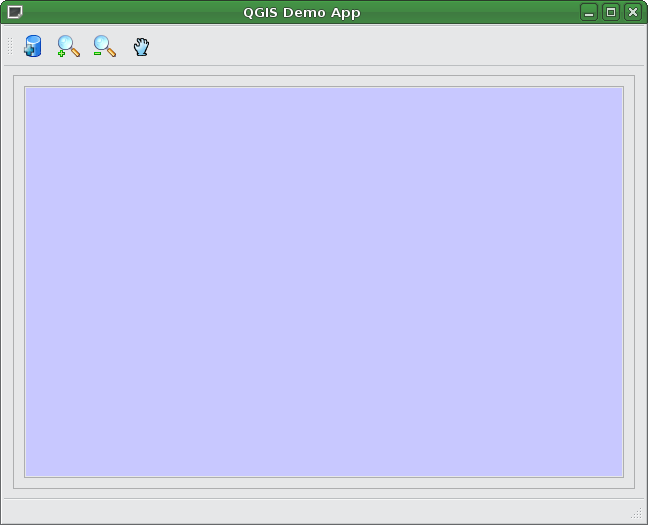
\includegraphics[clip=true, width=12cm]{python1_application}
\end{center}
\end{figure}

Για να προσθέσουμε το \filename{world\_borders} layer, κάνουμε κλικ στο εργαλείο
\usertext{Add Layer} και ανατρέχουμε στον κατάλογο δεδομένων.
Διαλέγουμε το shapefile και κάνουμε κλικ στο \button{Open} για να το προσθέσουμε στο χάρτη. 
Το προσωπικό χρώμα προστίθεται και το αποτέλεσμα φαίνεται στην Εικόνα \ref{fig:demo_app_done}.

Η δημιουργία μιας PyQGIS εφαρμογής είναι αρκετά απλή. Σε λιγότερο απο 150 γραμμές κώδικα έχουμε μία εφαρμογή που μπορεί να φορτώσει shapefile και να πλοηγηθεί στο χάρτη. Αν “παίξετε” λίγο με το χάρτη θα παρατηρήσετε ότι κάποια απο τα χαρακτηριστικά του κανβά επίσης δουλεύουν, συμπεριλαμβάνοντας και την πλοήγηση με τη ροδέλα του ποντικιού και τη μετακίνηση κρατώντας το \keystroke{Space} και κουνώντας το ποντίκι. 

SΚάποιες εξεζητημένες εφαρμογές έχουν δημιουργηθεί με PyQGIS και πολλές ακόμα δουλεύονται. Αυτό είναι αρκετά εντυπωσιακό, θεωρώντας ότι αυτή η ανάπτυξη ξεκίνησε ήδη πριν απο την επίσημη κυκλοφορία του QGIS 1.0.

\begin{figure}[ht]
\begin{center}
  \caption{Εικόνα 4: Προσθέτοντας ένα επίπεδο πληροφορίας στην demo εφαρμογή.\nixcaption} \label{fig:demo_app_done}
  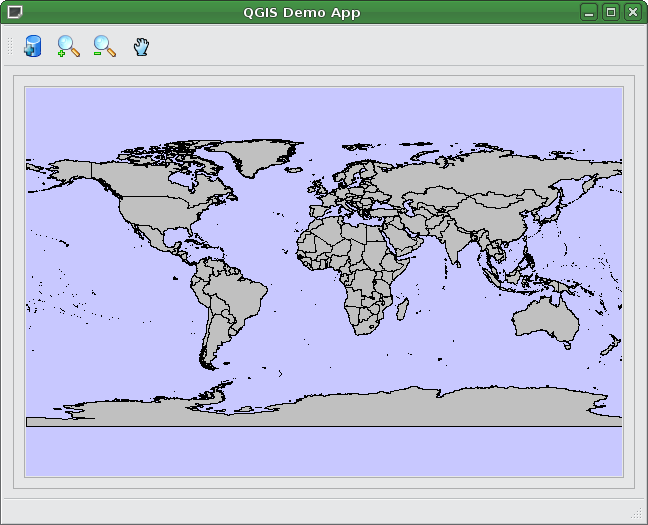
\includegraphics[clip=true, width=12cm]{python2_application}
\end{center}
\end{figure}

